\documentclass[ignorenonframetext,]{beamer}
\setbeamertemplate{caption}[numbered]
\setbeamertemplate{caption label separator}{: }
\setbeamercolor{caption name}{fg=normal text.fg}
\beamertemplatenavigationsymbolsempty
\usepackage{lmodern}
\usepackage{amssymb,amsmath}
\usepackage{ifxetex,ifluatex}
\usepackage{fixltx2e} % provides \textsubscript
\ifnum 0\ifxetex 1\fi\ifluatex 1\fi=0 % if pdftex
  \usepackage[T1]{fontenc}
  \usepackage[utf8]{inputenc}
\else % if luatex or xelatex
  \ifxetex
    \usepackage{mathspec}
  \else
    \usepackage{fontspec}
  \fi
  \defaultfontfeatures{Ligatures=TeX,Scale=MatchLowercase}
\fi
% use upquote if available, for straight quotes in verbatim environments
\IfFileExists{upquote.sty}{\usepackage{upquote}}{}
% use microtype if available
\IfFileExists{microtype.sty}{%
\usepackage{microtype}
\UseMicrotypeSet[protrusion]{basicmath} % disable protrusion for tt fonts
}{}
\newif\ifbibliography
\hypersetup{
            pdftitle={Final Project: Childhood Bullying and Subsequent Drug Use},
            pdfauthor={Shelley Facente, Steph Holm, Lizzy Kinnard, Veronica Pear},
            pdfborder={0 0 0},
            breaklinks=true}
\urlstyle{same}  % don't use monospace font for urls
\usepackage{longtable,booktabs}
\usepackage{caption}
% These lines are needed to make table captions work with longtable:
\makeatletter
\def\fnum@table{\tablename~\thetable}
\makeatother
\usepackage{graphicx,grffile}
\makeatletter
\def\maxwidth{\ifdim\Gin@nat@width>\linewidth\linewidth\else\Gin@nat@width\fi}
\def\maxheight{\ifdim\Gin@nat@height>\textheight0.8\textheight\else\Gin@nat@height\fi}
\makeatother
% Scale images if necessary, so that they will not overflow the page
% margins by default, and it is still possible to overwrite the defaults
% using explicit options in \includegraphics[width, height, ...]{}
\setkeys{Gin}{width=\maxwidth,height=\maxheight,keepaspectratio}

% Prevent slide breaks in the middle of a paragraph:
\widowpenalties 1 10000
\raggedbottom

\AtBeginPart{
  \let\insertpartnumber\relax
  \let\partname\relax
  \frame{\partpage}
}
\AtBeginSection{
  \ifbibliography
  \else
    \let\insertsectionnumber\relax
    \let\sectionname\relax
    \frame{\sectionpage}
  \fi
}
\AtBeginSubsection{
  \let\insertsubsectionnumber\relax
  \let\subsectionname\relax
  \frame{\subsectionpage}
}

\setlength{\parindent}{0pt}
\setlength{\parskip}{6pt plus 2pt minus 1pt}
\setlength{\emergencystretch}{3em}  % prevent overfull lines
\providecommand{\tightlist}{%
  \setlength{\itemsep}{0pt}\setlength{\parskip}{0pt}}
\setcounter{secnumdepth}{0}

\title{Final Project: Childhood Bullying and Subsequent Drug Use}
\author{Shelley Facente, Steph Holm, Lizzy Kinnard, Veronica Pear}
\date{Spring 2019}

\begin{document}
\frame{\titlepage}

\section{Causal Question: What is the effect of having been bullied
prior to age 12 on incidence of drug use in adolescence or
adulthood?}\label{causal-question-what-is-the-effect-of-having-been-bullied-prior-to-age-12-on-incidence-of-drug-use-in-adolescence-or-adulthood}

\begin{frame}{Specify a Causal Model}

Our dataset:

\begin{itemize}
\tightlist
\item
  National Longitudinal Survey of Youth
\item
  Nationally representative cohort of youth age 12-16
\item
  Initial recruitment n = 9000 in 1997
\item
  In our final dataset n = 7703
\end{itemize}

\end{frame}

\begin{frame}{Original DAG}

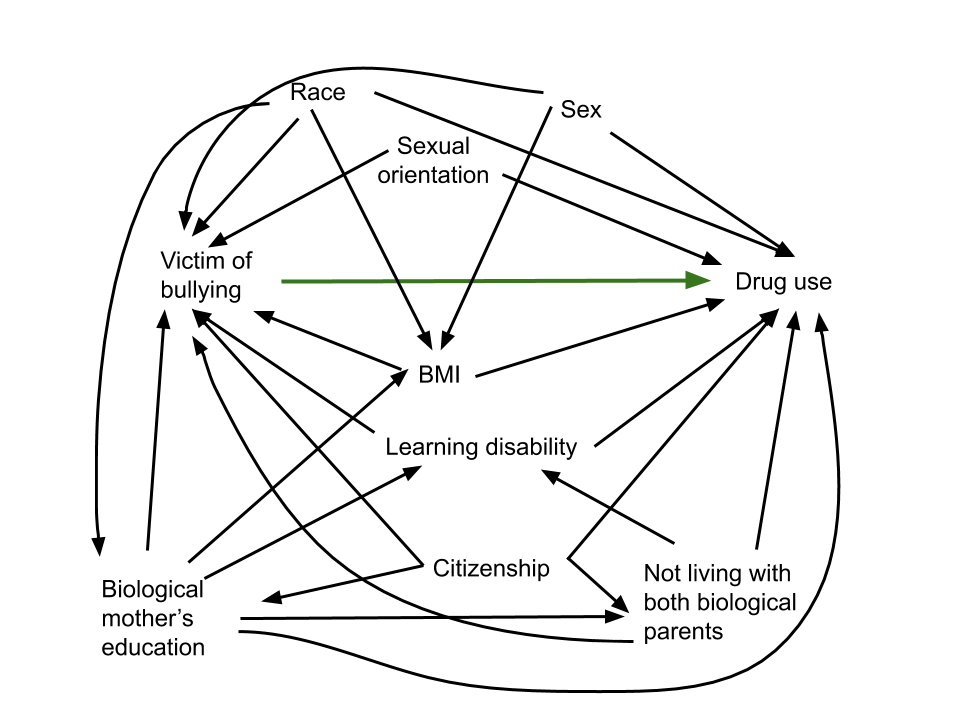
\includegraphics[width=1\linewidth]{DAG Causal Final Project_all covariates}

\end{frame}

\begin{frame}{Final DAG}

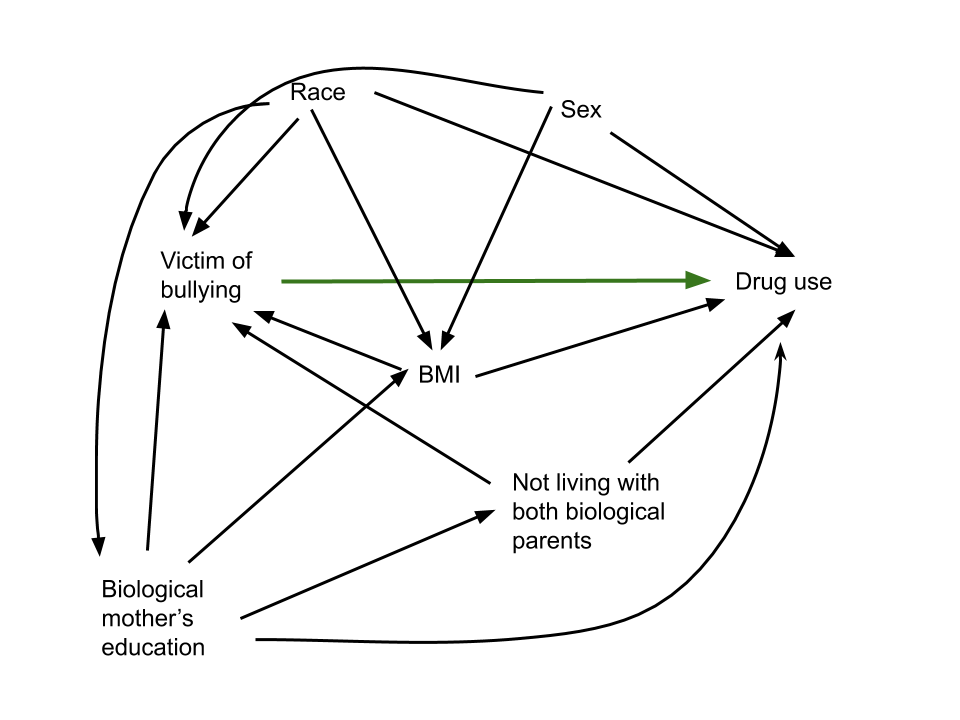
\includegraphics[width=1\linewidth]{DAG Causal Final Project_reduced covariates}

\end{frame}

\begin{frame}{Structural Equations}

Our endogenous nodes include: \(X = (W, A, Y)\), where
\(W = (W_1, W_2, W_3, W_4, W_5)\) is the set of baseline covariates,
\(A\) is victim of bullying, and \(Y\) is incident drug use.

\vspace{12pt}

Our background variables (exogenous nodes) include:
\(U = (U_W, U_A, U_Y)\) \textasciitilde{} \(\mathbb{P}_U\).

\vspace{12pt}

We place no assumptions on the distribution \(\mathbb{P}_U\). We have
not placed any restrictions on the functional form.

\end{frame}

\begin{frame}{Structural Equations}

Our structural equations \(\mathcal{F}\) are:

\[
\begin{aligned}
W_1 &= f_{W_1} (U_{W_1}, W_3) \\
W_2  &= f_{W_2}  (U_{W_2}) \\
W_3  &= f_{W_3}  (U_{W_3}) \\
W_4  &= f_{W_4} (U_{W_4}, W_1) \\
W_5  &= f_{W_5} (U_{W_5}, W_1, W_2, W_3) \\
A &= f_A (U_A, W_1, W_2, W_3, W_4, W_5) \\
Y &= f_Y (U_Y, A, W_1, W_2, W_3, W_4, W_5) \\
\end{aligned}
\]

\vspace{12pt}

Where \(W_1\) = mother's education; \(W_2\) = sex; \(W_3\) =
race/ethnicity; \(W_4\) = not living with both biological parents;
\(W_5\) = BMI z-score; \(A\) = bullied before the age of 12 (asked in
1997); \(Y\) = incident drug use (``cocaine or other hard drugs'') after
1997.

\end{frame}

\begin{frame}{Target Causal Parameter}

Our target causal parameter is the difference in the counterfactual
probability of drug use if all kids were bullied prior to age 12, and
the counterfactual probability of drug use if all kids were not bullied
prior to age 12:

\[
\psi^F (P_{U,X}) = P_{U,X} (Y_1 = 1) - P_{{U,X}}(Y_0=1) = E_{U,X}(Y_1) - E_{U,X}(Y_0)
\] where \(Y_a\) denotes the counterfactual outcome under an
intervention to set bullying status A = a. This target causal parameter
is the average treatment effect (ATE), or causal risk difference.

\end{frame}

\begin{frame}{Link to the SCM}

We assume that the observed data O = (W, A, Y) \textasciitilde{}
\(\mathbb{P}_0\) were generated by sampling n times from a data
generating process described by the SCM. The statistical model
\(\mathcal{M}\) for the set of allowed distributions for the observed
data is non-parametric.

\end{frame}

\begin{frame}{Table 1}

\fontsize{8}{8} \selectfont 

\begin{longtable}[]{@{}lll@{}}
\toprule
Covariate & Drug use (\%) & No drug use (\%)\tabularnewline
\midrule
\endhead
\(\textbf{Drug use (Total)}\) & 1330 (17.3\%) & 6373
(82.7\%)\tabularnewline
& &\tabularnewline
\(\textbf{Victim of bullying}\) & &\tabularnewline
Yes & 319 (4.1\%) & 1179 (15.3\%)\tabularnewline
No & 1011 (13.1\%) & 5194 (67.4\%)\tabularnewline
& &\tabularnewline
\(\textbf{Mother's education}\) & &\tabularnewline
High school or less & 3867 (50.2\%) & 732 (9.5\%)\tabularnewline
Some college or more & 598 (7.8\%) & 2506 (32.5\%)\tabularnewline
& &\tabularnewline
\(\textbf{Sex}\) & &\tabularnewline
Female & 591 (7.7\%) & 3218 (41.8\%)\tabularnewline
Male & 739 (9.6\%) & 3155 (41\%)\tabularnewline
& &\tabularnewline
\(\textbf{Race/ethnicity}\) & &\tabularnewline
Black & 227 (2.9\%) & 1788 (23.2\%)\tabularnewline
Hispanic & 288 (3.7\%) & 1340 (17.4\%)\tabularnewline
Non-Black, Non-Hispanic & 815 (10.6\%) & 3245 (42.1\%)\tabularnewline
& &\tabularnewline
\(\textbf{Living with both biological parents}\) & &\tabularnewline
Yes & 645 (8.4\%) & 3176 (41.2\%)\tabularnewline
No & 685 (8.9\%) & 3197 (41.5\%)\tabularnewline
& &\tabularnewline
\(\textbf{BMI z-score}\) & 0.513 (\emph{mean}) & 0.505
(\emph{mean})\tabularnewline
\textcolor{white}{x} & 1.03 (\emph{sd}) & 0.98
(\emph{sd})\tabularnewline
\bottomrule
\end{longtable}

\end{frame}

\begin{frame}{Identifiability}

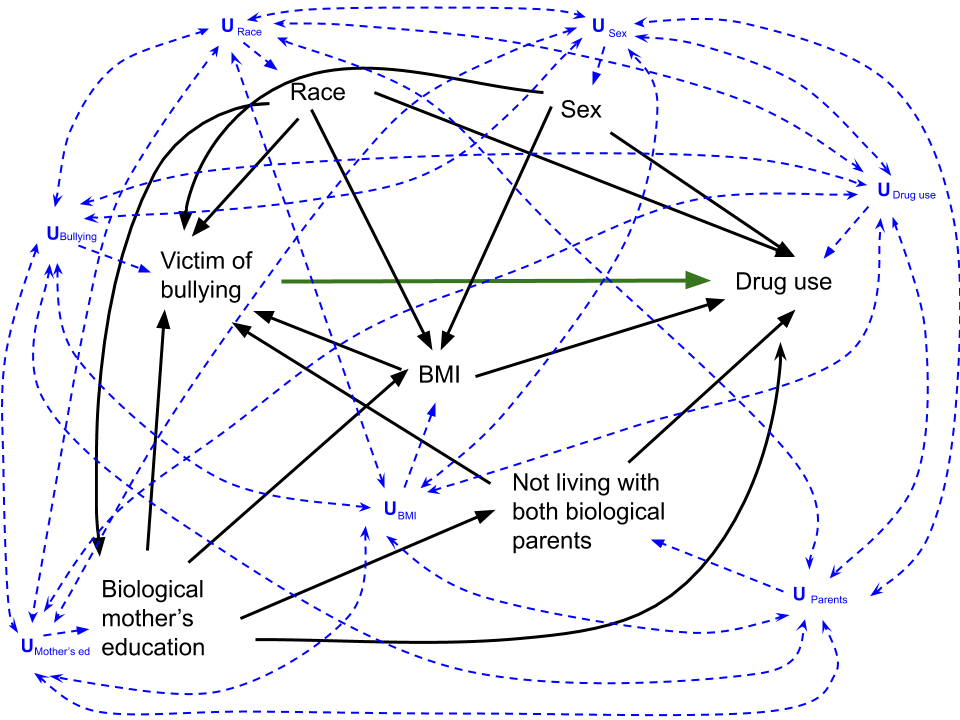
\includegraphics[width=1\linewidth]{DAG Causal Final Project_reduced covariates with Us}

\end{frame}

\begin{frame}{Identifiability}

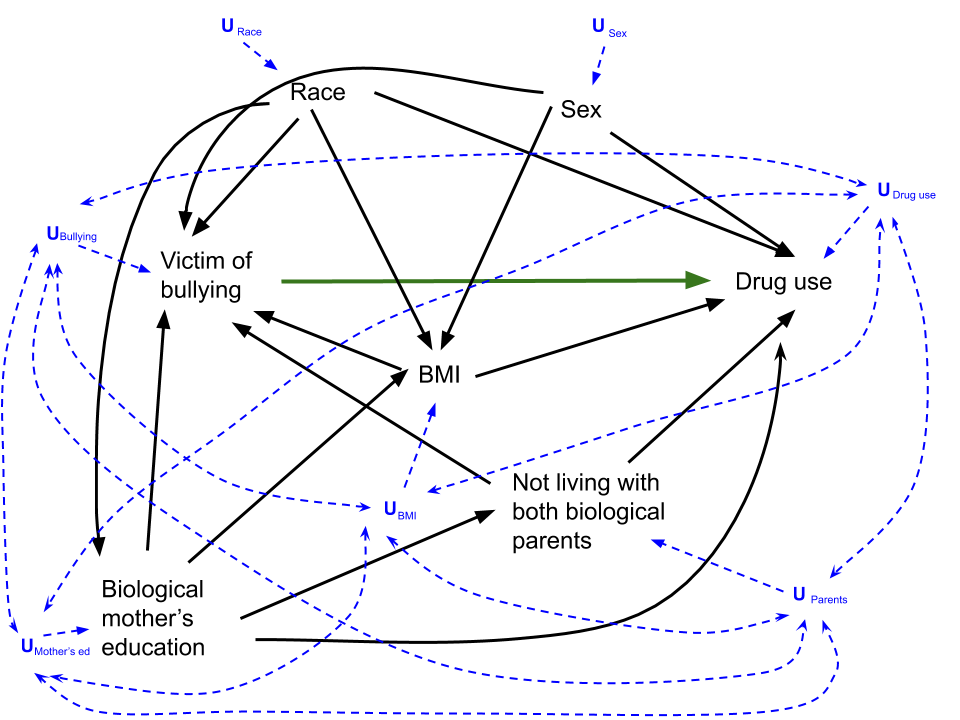
\includegraphics[width=1\linewidth]{DAG Causal Final Project_reduced covariates with Us_reality}

\end{frame}

\begin{frame}{Identifiability}

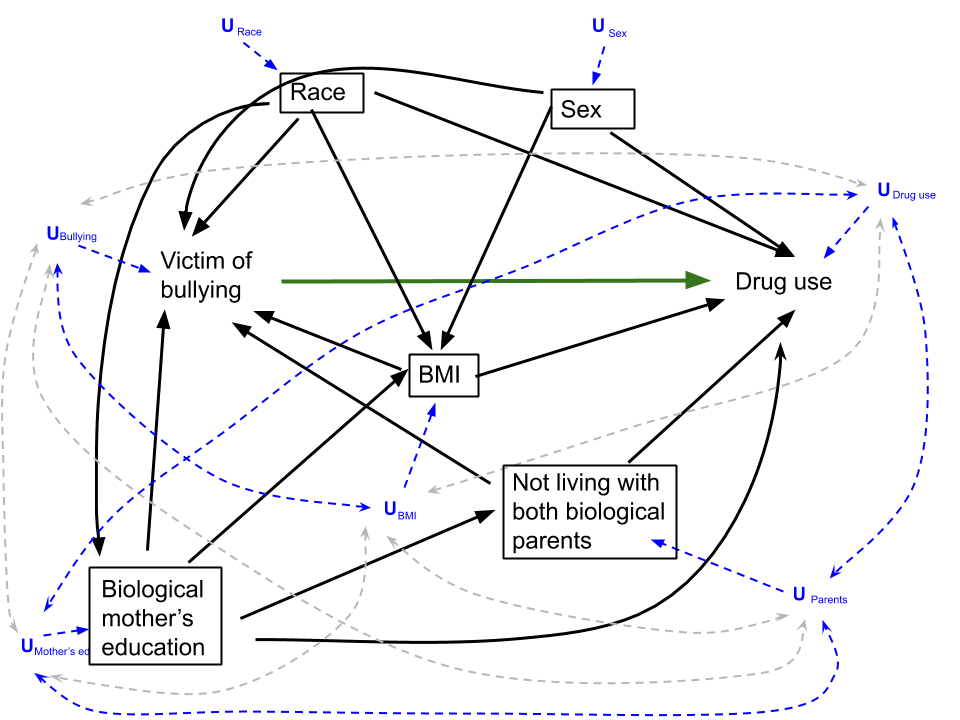
\includegraphics[width=1\linewidth]{DAG Causal Final Project_reduced covariates with Us_convenience}

\end{frame}

\begin{frame}{Identifiability}

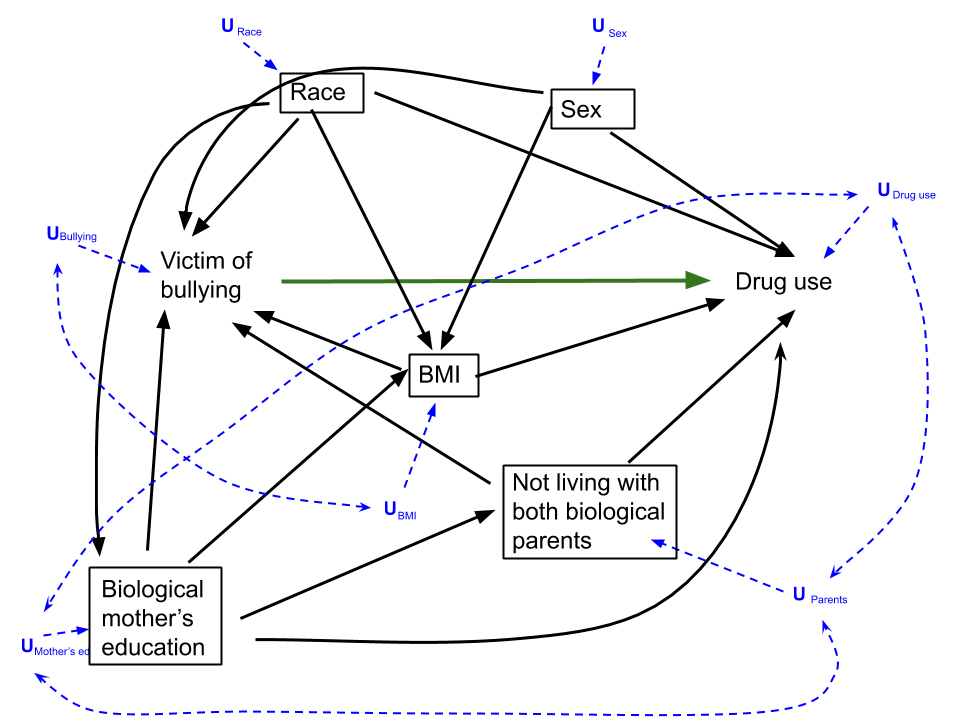
\includegraphics[width=1\linewidth]{DAG Causal Final Project_reduced covariates with Us_final}

\end{frame}

\begin{frame}{Estimand and Statistical Model}

The target parameter of the observed data distribution (which equals the
causal parameter in the augmented causal model \(\mathcal{M}^{F\star}\))
is the G-Computation formula:

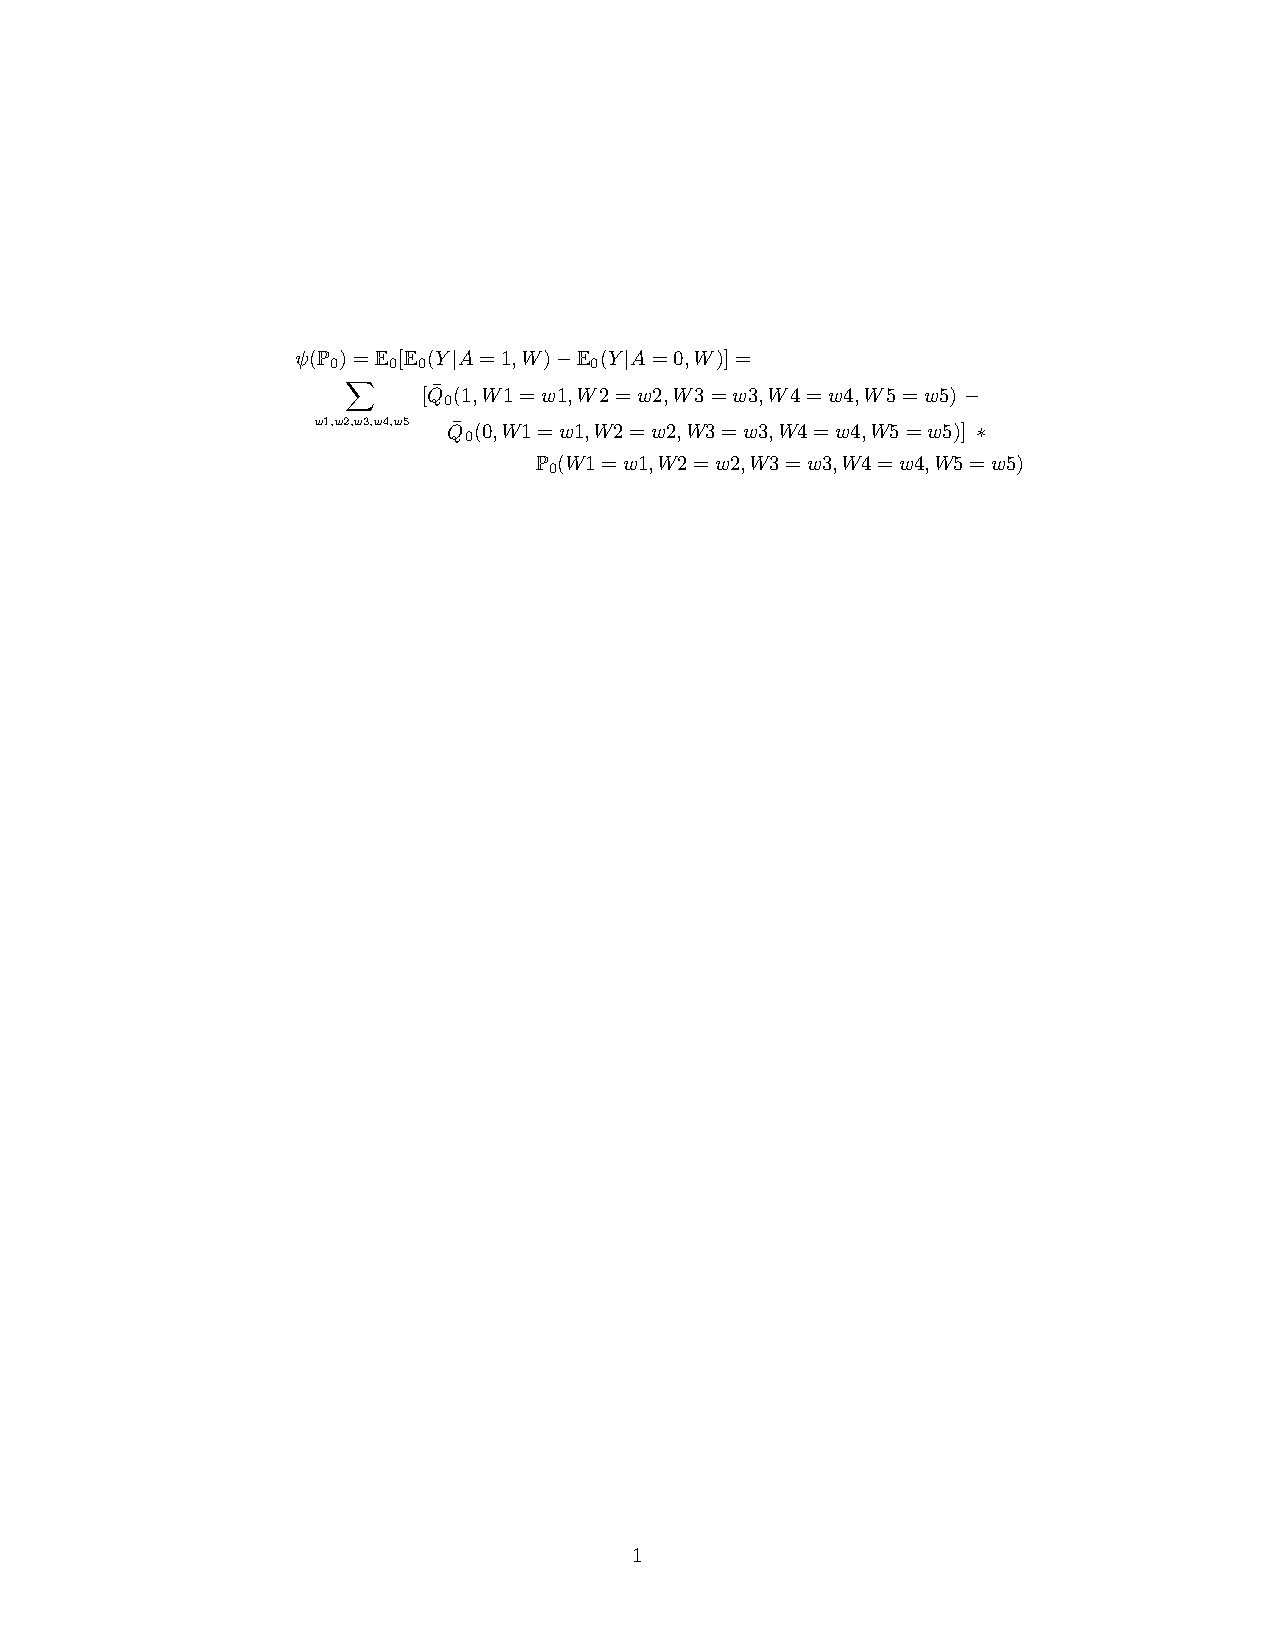
\includegraphics[width=14.99in]{estimand}

This is our statistical estimand.

\end{frame}

\begin{frame}{Checking for Practical Positivity Violations}

\begin{itemize}
\item
  We tabulated exposure and outcome across all possible levels of our
  categorical variables
\item
  Observations exist in every possible category of our variable set
\item
  For our only continuous variable, BMI z-score (for age and sex), we
  looked at the distribution of BMI z-scores in the two exposure
  categories
\end{itemize}

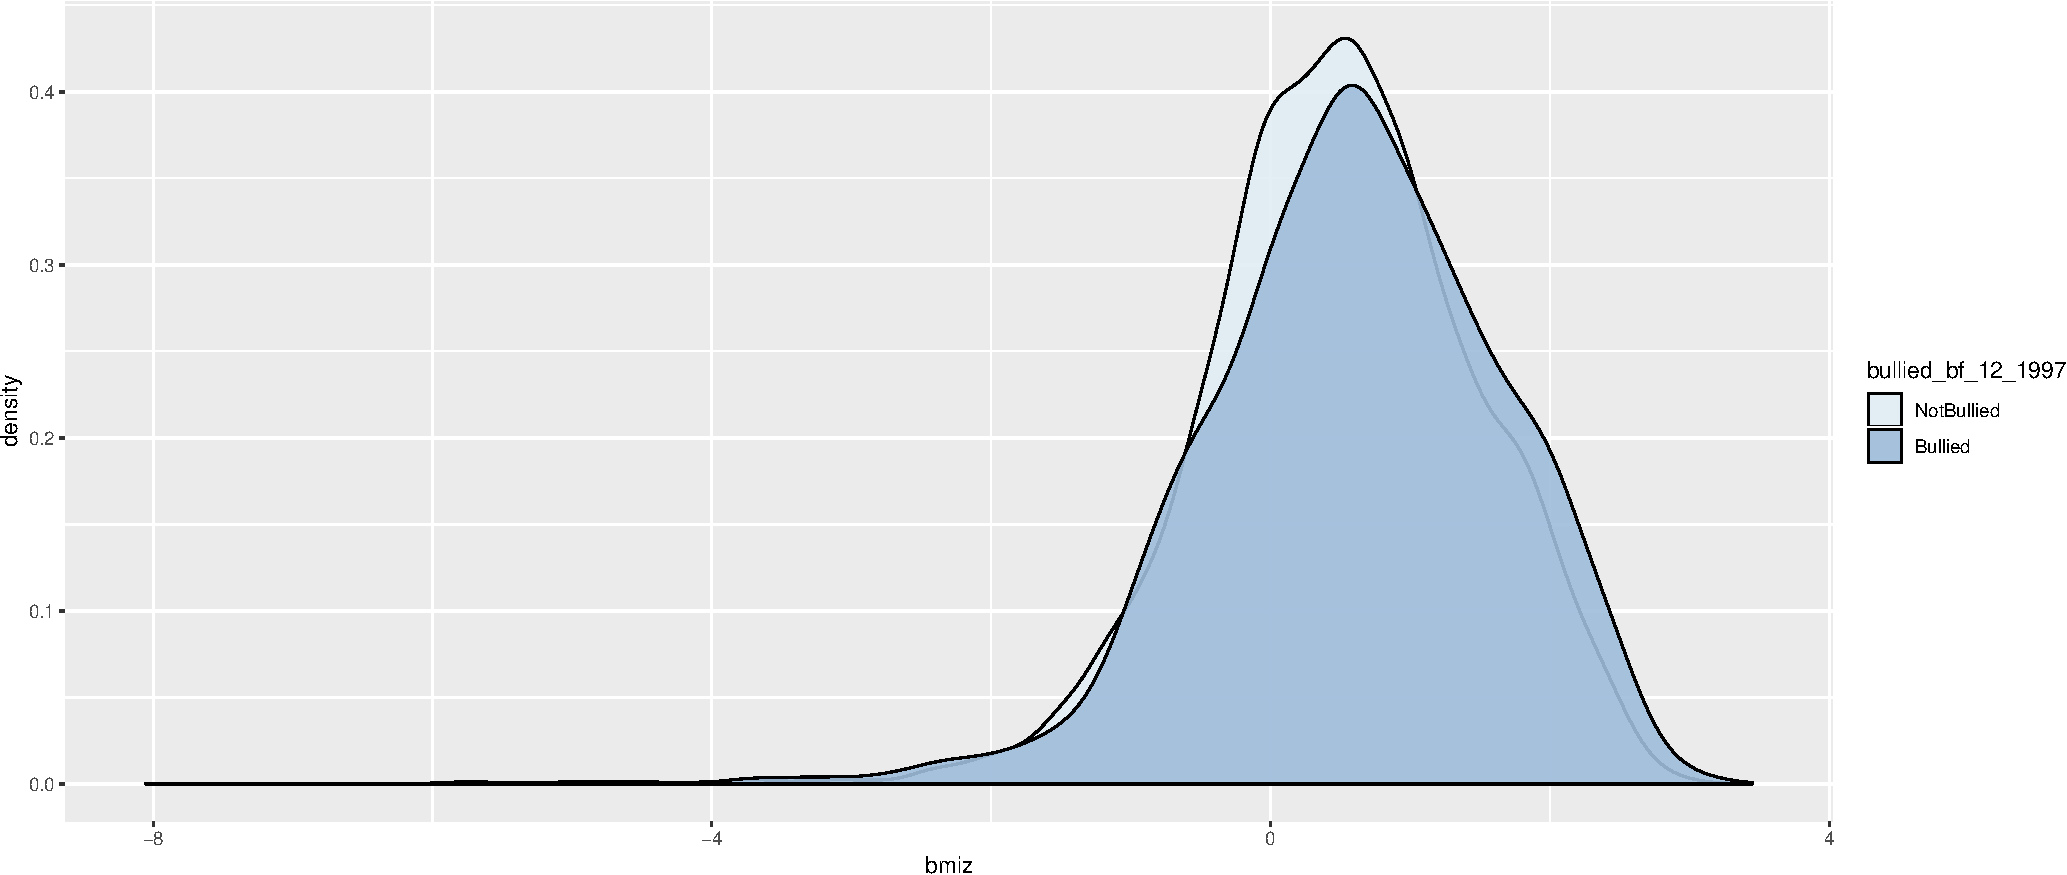
\includegraphics{Final_Project_Coding_files/figure-beamer/unnamed-chunk-2-1.pdf}

\end{frame}

\begin{frame}{Positivity: Assessing the Model Weights}

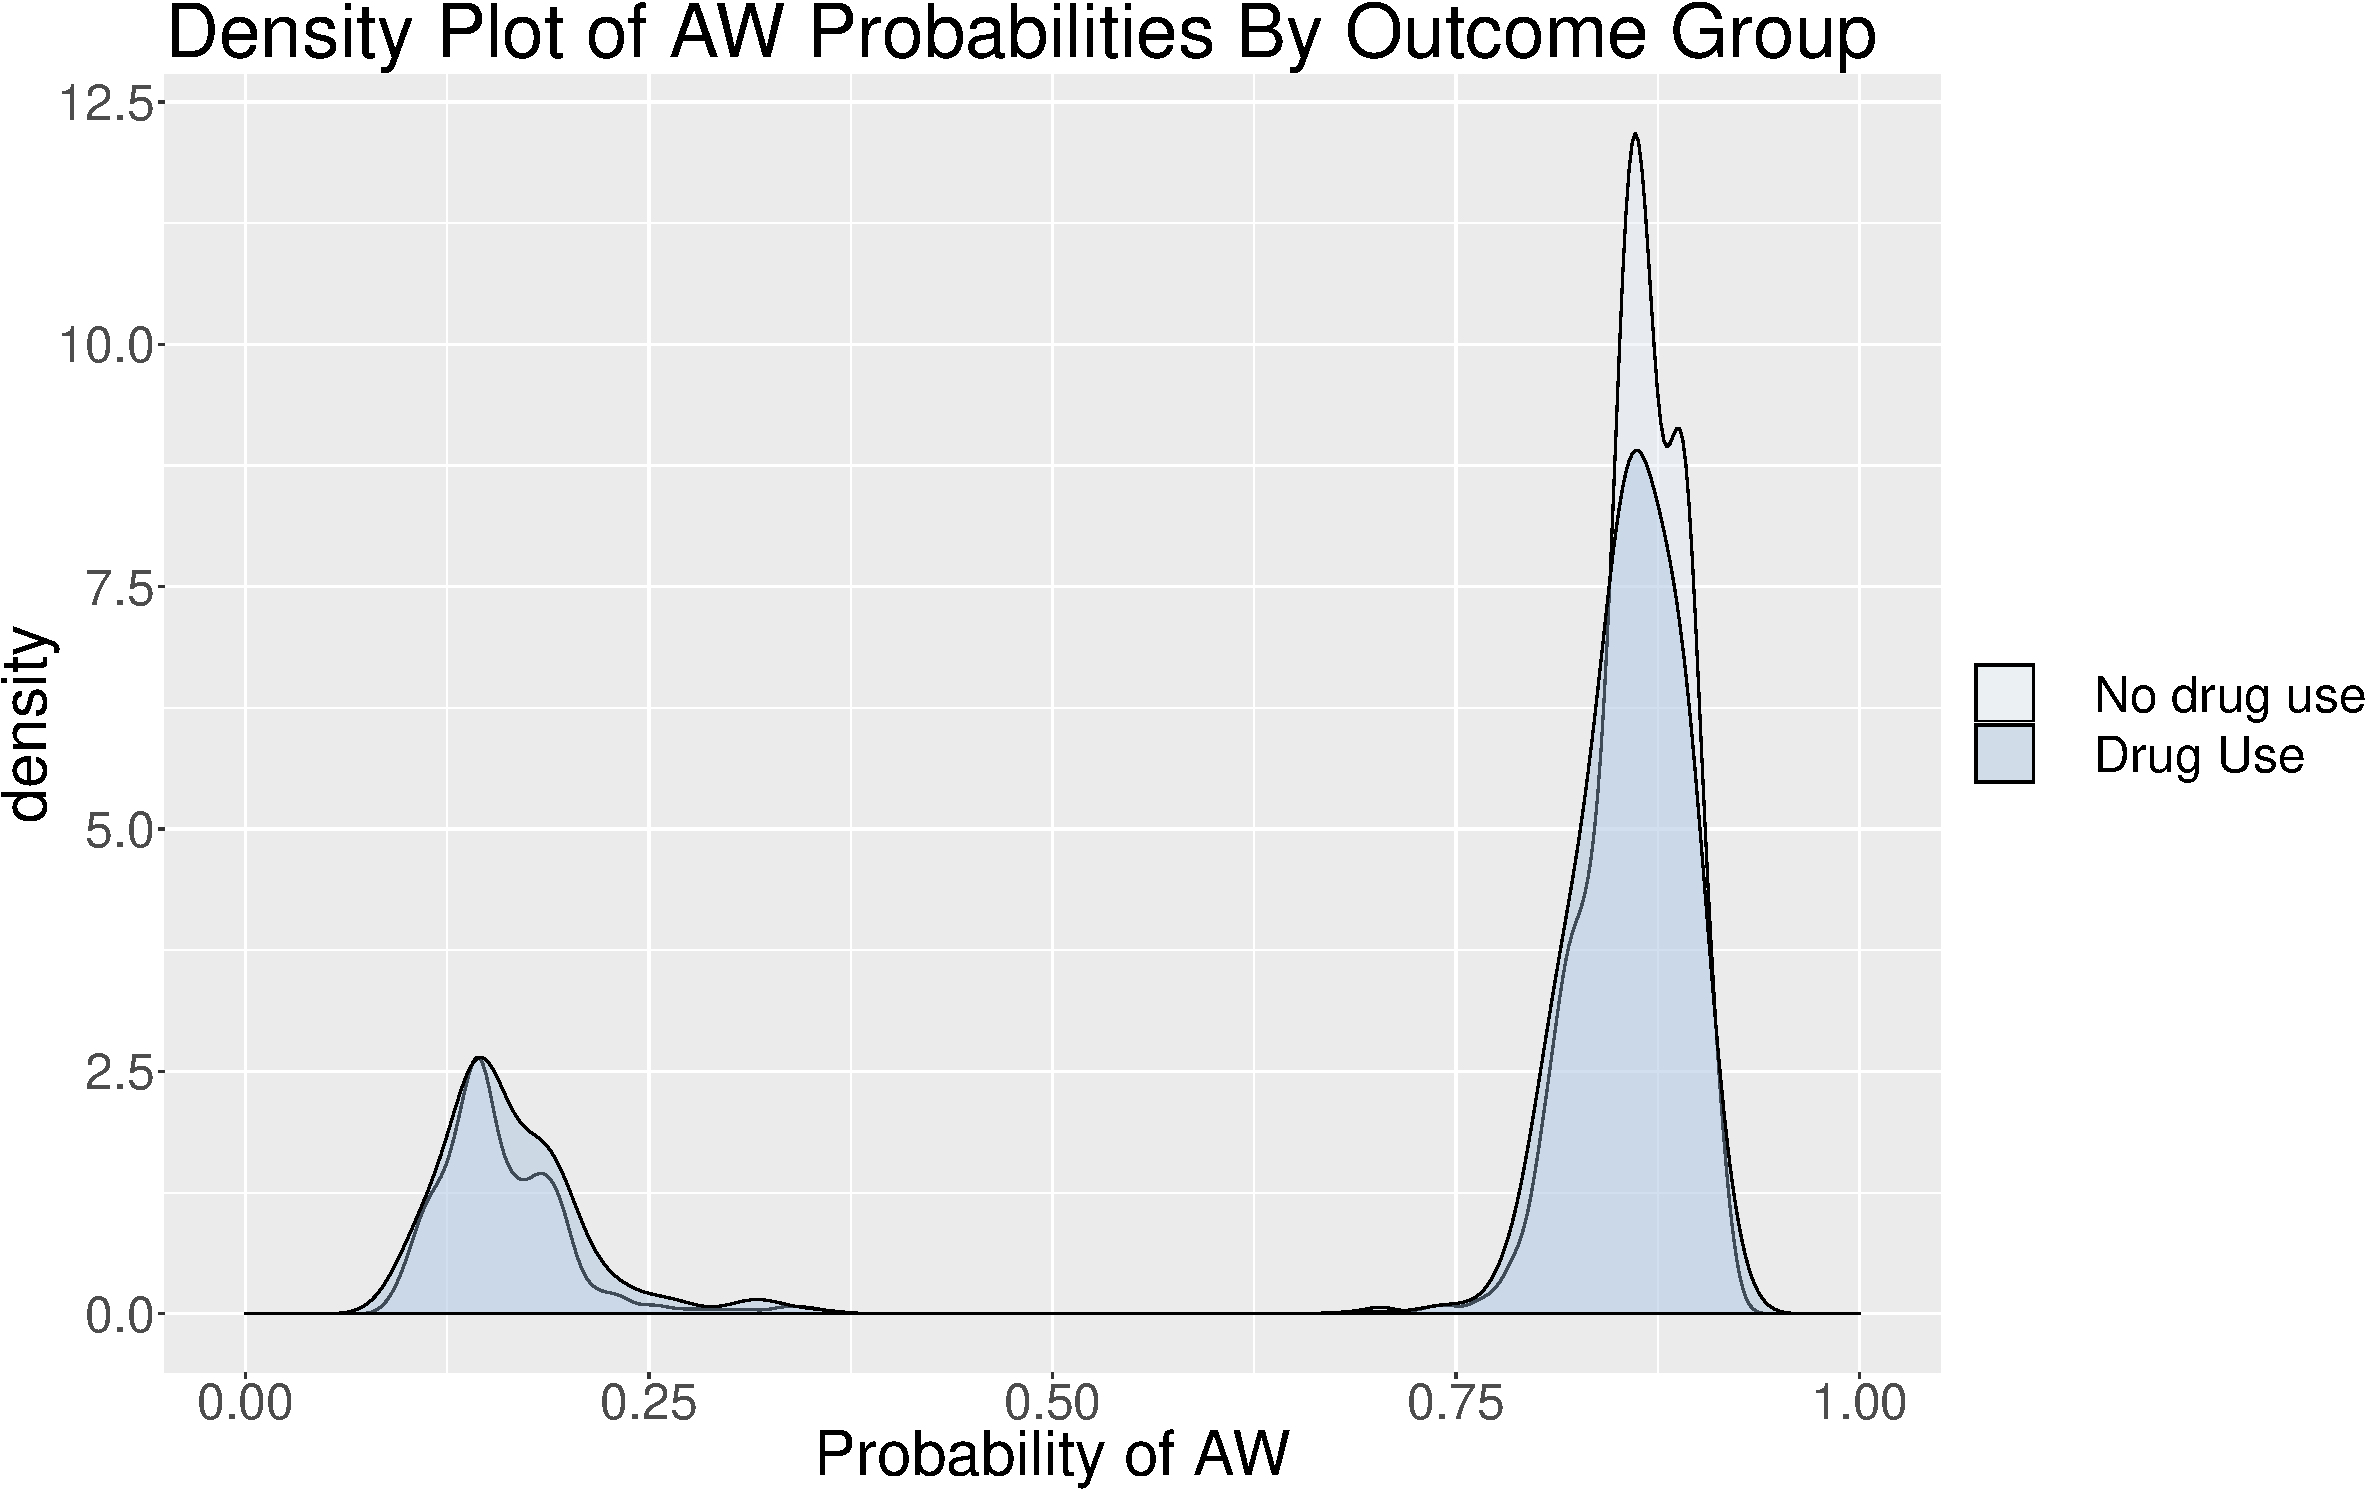
\includegraphics{Final_Project_Coding_files/figure-beamer/unnamed-chunk-3-1.pdf}

\end{frame}

\begin{frame}{Estimation}

\begin{itemize}
\item
  We use SuperLearner for prediction in all models.
\item
  Library: SL.glm, SL.glm.interaction, SL.glmnet, SL.bayesglm,
  SL.randomForest, SL.step, SL.mean
\item
  5-fold cross-validation
\item
  We use the following estimators: G-computation (simple substituion
  estimator), stabilized IPTW, and TMLE
\end{itemize}

\end{frame}

\begin{frame}{Confidence Intervals}

\begin{itemize}
\item
  For TMLE, used the robust method built in to the ltmle package
\item
  For G-comp and IPTW we performed a bootstrap
\end{itemize}

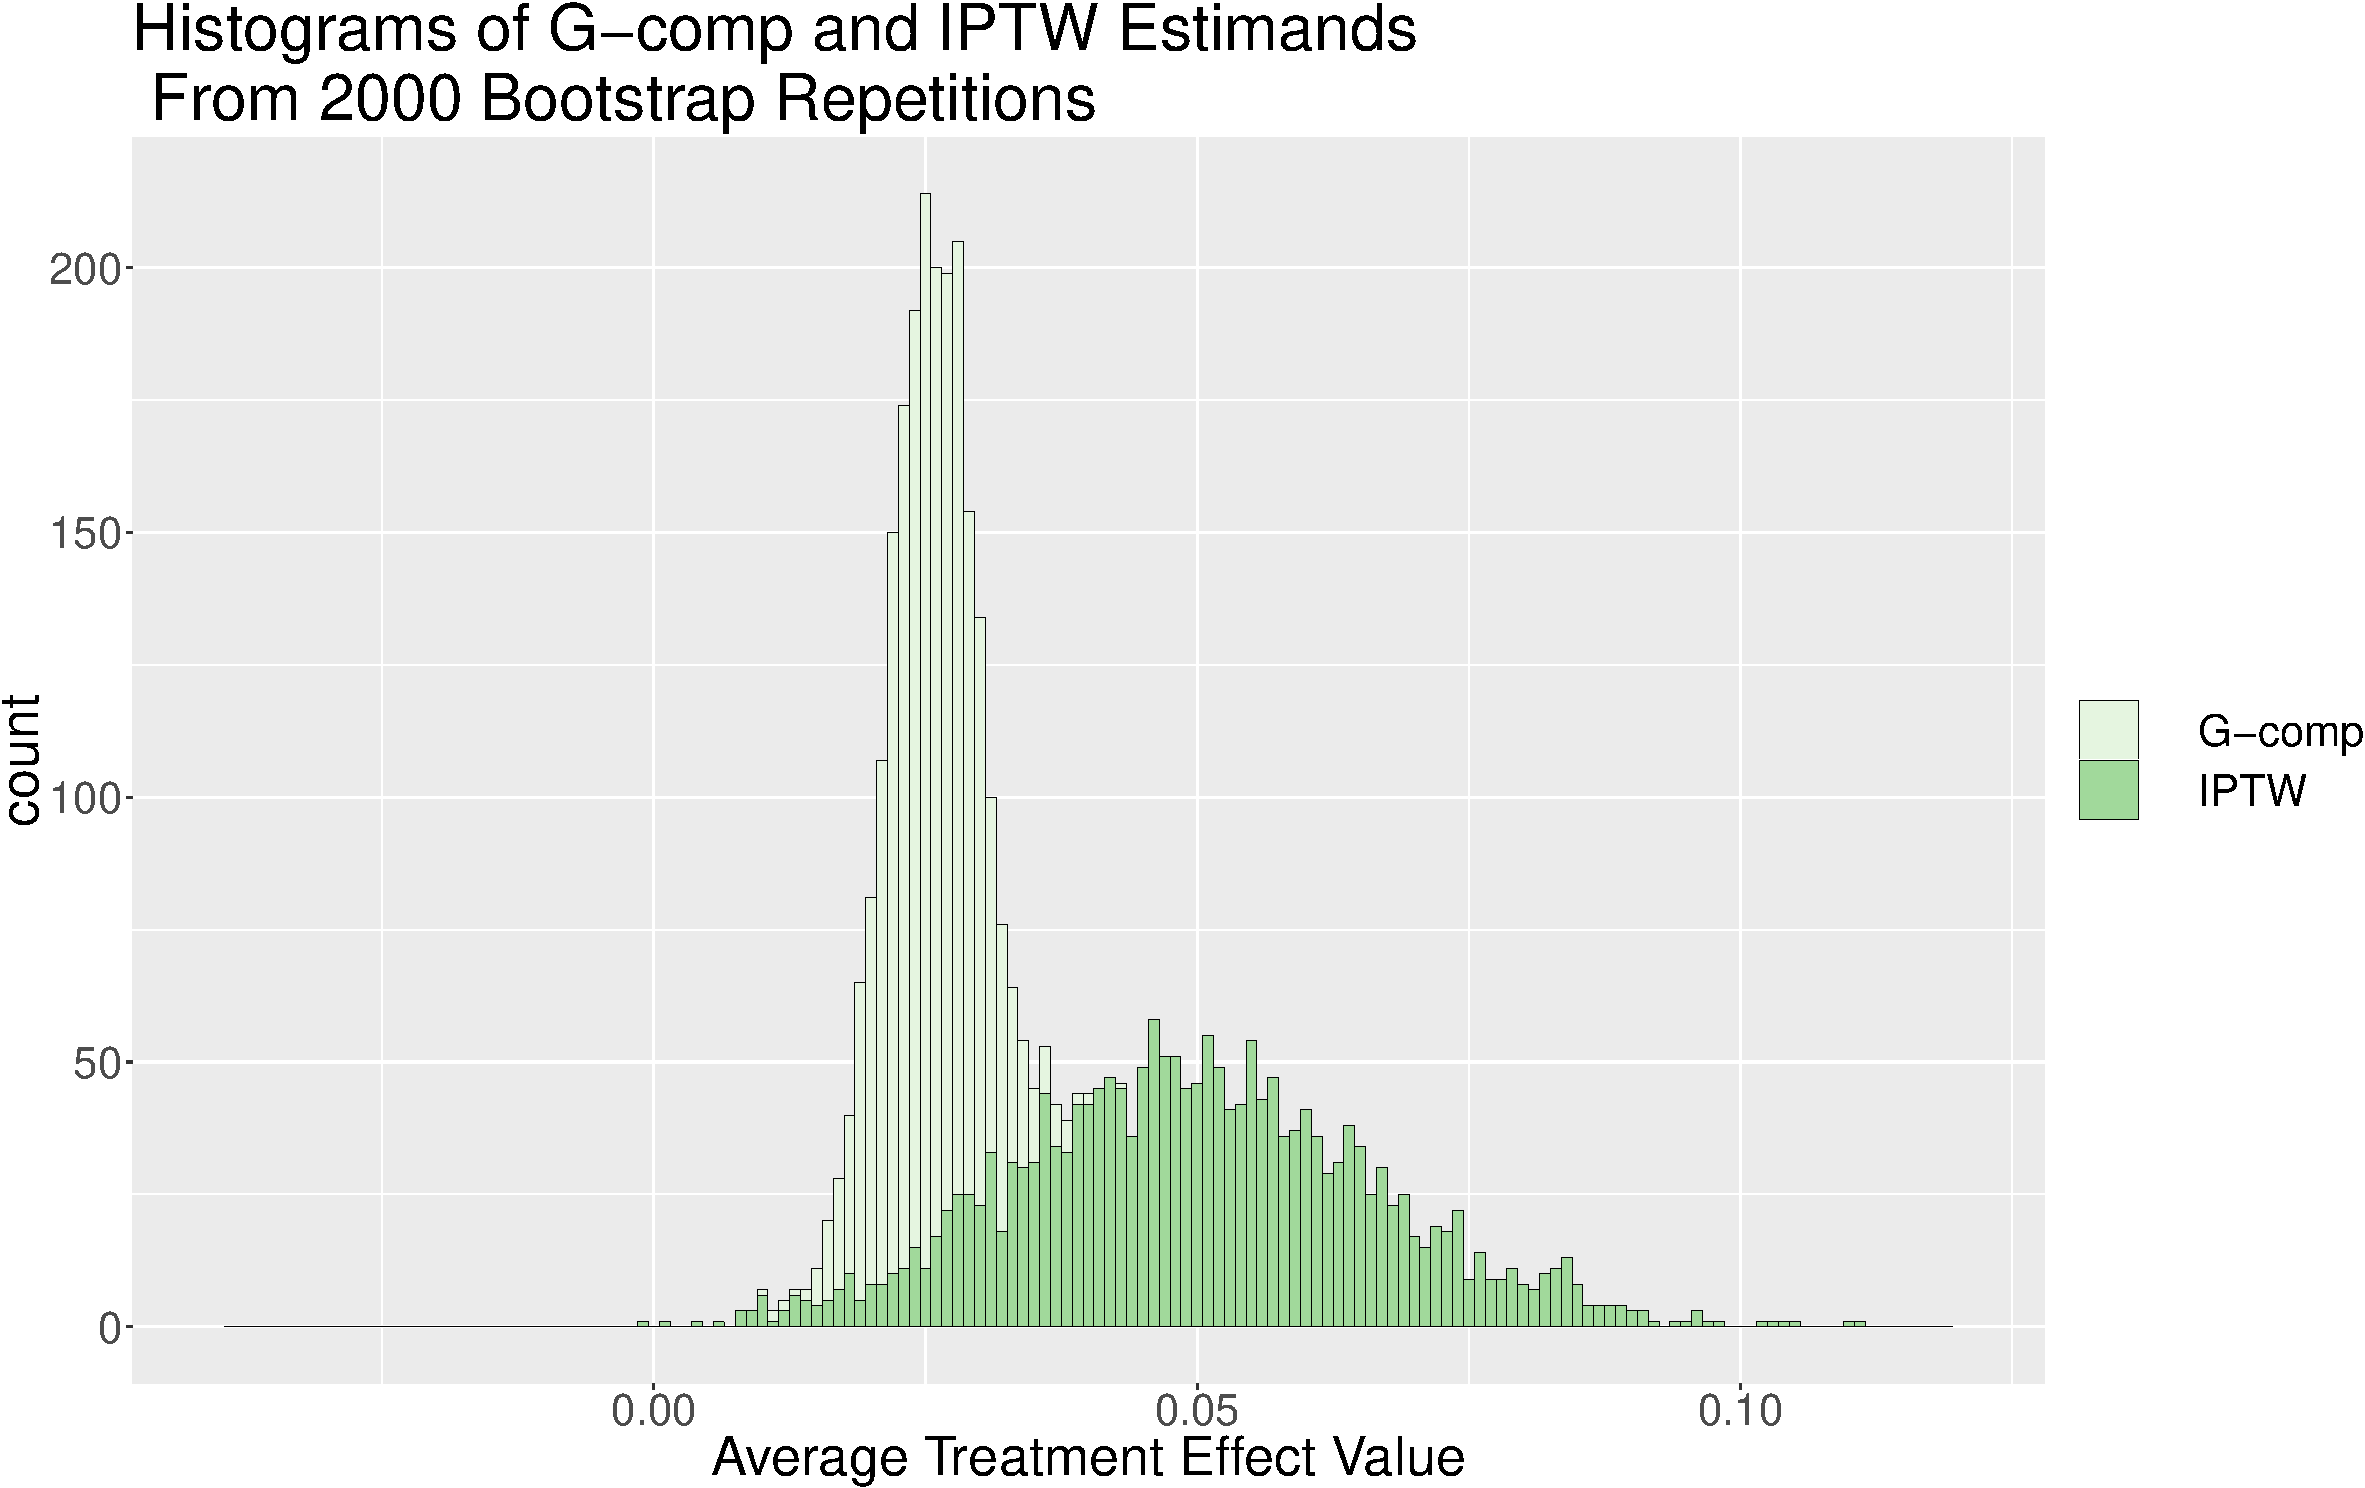
\includegraphics{Final_Project_Coding_files/figure-beamer/unnamed-chunk-4-1.pdf}

\end{frame}

\begin{frame}{Estimation}

\begin{longtable}[]{@{}ll@{}}
\toprule
Estimator & ATE (95\% CI)\tabularnewline
\midrule
\endhead
G-computation & 0.039 (0.017, 0.034)\tabularnewline
Stabilized IPTW & 0.045 (0.018, 0.084)\tabularnewline
TMLE & 0.044 (0.007, 0.08)\tabularnewline
\bottomrule
\end{longtable}

\begin{itemize}
\tightlist
\item
  The unadjusted ATE = mean(Y\textbar{}A=1 - Y\textbar{}A=0) = 0.05
\end{itemize}

\end{frame}

\begin{frame}{Estimation: SuperLearner convex combinations}

\begin{longtable}[]{@{}lllll@{}}
\toprule
Algorithm & A Risk & A Coefficient & Y Risk & Y
Coefficient\tabularnewline
\midrule
\endhead
glm & 0.155 & 0 & 0.1409 & 0.4629\tabularnewline
glm.interaction & 0.1551 & 0.2087 & 0.1415 & 0\tabularnewline
glmnet & 0.155 & 0 & 0.1409 & 0\tabularnewline
bayesglm & 0.155 & 0 & 0.1409 & 0\tabularnewline
randomForest & 0.1903 & 0.4607 & 0.1707 & 0.224\tabularnewline
step & 0.1549 & 0.2676 & 0.1409 & 0.2477\tabularnewline
mean & 0.1567 & 0.063 & 0.1429 & 0.0655\tabularnewline
\bottomrule
\end{longtable}

\end{frame}

\begin{frame}{Estimation: SuperLearner performance}

CV.SuperLearner

\begin{longtable}[]{@{}lll@{}}
\toprule
Algorithm & Avg Risk & SE\tabularnewline
\midrule
\endhead
SuperLearner & 0.1412 & 0.0029\tabularnewline
Discrete SL & 0.1407 & 0.0028\tabularnewline
glm & 0.1407 & 0.0028\tabularnewline
glm.interaction & 0.1413 & 0.0028\tabularnewline
glmnet & 0.1407 & 0.0028\tabularnewline
bayesglm & 0.1407 & 0.0028\tabularnewline
randomForest & 0.1679 & 0.0042\tabularnewline
step & 0.1407 & 0.0028\tabularnewline
mean & 0.1429 & 0.0028\tabularnewline
\bottomrule
\end{longtable}

\end{frame}

\begin{frame}{Interpretation}

According to our analysis:

\begin{itemize}
\item
  the difference between the average counterfactual risk of drug use if
  everyone was bullied versus if no one was bullied is 0.04
\item
  \textbf{causal interpretation}: if people are bullied, they have about
  a 4\% increased likelihood of drug use later in life than people who
  are not bullied
\end{itemize}

\begin{longtable}[]{@{}ll@{}}
\toprule
Estimator & ATE (95\% CI)\tabularnewline
\midrule
\endhead
G-computation & 0.039 (0.017, 0.034)\tabularnewline
Stabilized IPTW & 0.045 (0.018, 0.084)\tabularnewline
TMLE & 0.044 (0.007, 0.08)\tabularnewline
\bottomrule
\end{longtable}

\end{frame}

\begin{frame}{Limitations}

\begin{enumerate}
\def\labelenumi{\arabic{enumi}.}
\tightlist
\item
  Important exogenous variables\\

  \begin{itemize}
   \item Parent drug use 
   \item Mental health 
   \item And more...
     \end{itemize}
\item
  Necessary independence assumptions
\end{enumerate}

\end{frame}

\begin{frame}{Impacts}

\begin{itemize}
\item
  Identify youth who are at risk for starting to use drugs as a result
  of bullying
\item
  Supports use of anti-bullying interventions in schools
\end{itemize}

\end{frame}

\begin{frame}{Contributions of the Team Members}

\begin{itemize}
\item
  Suggestion of a dataset and potential issues for exploration: Veronica
\item
  Particular expertise that we each contributed:

  \begin{enumerate}
   \item Shelley - Project management
   \item Stephanie - Pediatrics 
   \item Veronica - Social and Substance Use Epi
   \item Lizzy - Social and Substance Use Epi
     \end{enumerate}
\item
  Establishment of the causal model, delineation of the causal question
  and estimand of choice: Entire group
\item
  Identifiability considerations: Entire group, with Lizzy and Shelley
  working on the DAG
\item
  Creation of slides for causal question, SCM, background on our
  dataset: Lizzy and Shelley
\item
  Creation of SuperLearner library: Veronica
\item
  Coding of ATE point estimates: Veronica
\item
  Coding of Practical Positivity Checks and Bootstrapping of Confidence
  Intervals: Stephanie
\item
  Interpretation of Results: Entire Group
\end{itemize}

\end{frame}

\end{document}
